\chapter{Flowsheeting}

\begin{overview}
  Even though many representations of chemical processes are possible
  in theory, the flowsheet is the most popular in practice.  Process
  engineers use process flow diagrams and piping and instrumentation
  diagrams to document processes and flowsheeting software leverages
  their familiarity with the flowsheet format to represent the
  processes being simulated.  An overview is given here of
  flowsheeting terminology and common unit operations, along with
  common methods of solving dynamic and stationary flowsheeting
  problems.
\end{overview}

\section{Unit operations}
The concept of unit operations has been embedded in Chemical
Engineers' psyche since Arthur D. Little coined the phrase in
1915~\citep{hougenhistory}.  Unit operations lend themselves to an
object-oriented programming style, with their main functions
encapsulated in a ``black box'', with narrow interfaces between them.
The following main unit operations are identified, following the
sequence used in~\citet{msh}.

\subsection{Fluid flow operations}
These operations are further subdivided based on the nature of the
fluid flowing in them.  Uncompressible and compressible single phase
flow are the most commonly modelled types; multiphase flow is commonly
encountered in industry, but presents significant modelling
challenges.\citehere.

\subsubsection{Fluid movers}
This category encapsulates pumps, blowers, compressors and similar
equipment which bring about a change in momentum of a fluid by doing
work on it.  

\subsubsection{Valves}


\subsubsection{Pipes}


\subsection{Heat transfer}
\subsubsection{Heat exchangers}


\subsection{VLE}
Mass transfer operations 


%% Mention something about the phase rule and degrees of freedom

\subsubsection{Flashing}
A flash drum is a unit that separates a stream into a vapour and
liquid fraction based on the difference in composition of vapour and
liquid in phase equilibrium.  Figure~\ref{fig:flashdrum} shows a flash
drum with the relevant variables.

\begin{figure}[htbp]
  \centering
  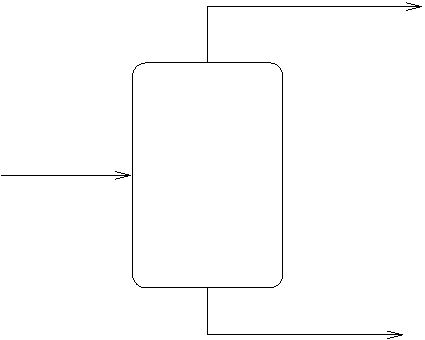
\includegraphics[width=0.4\textwidth]{flashdrum}
  \caption{Flash drum}
  \label{fig:flashdrum}
\end{figure}

The following assumptions are common when modelling flash drums:

\begin{itemize}
\item The phase equilibrium is achieved fully and quickly relative to
  the dynamics of the level of the flash drum.
\item The pressure in the flash drum changes only due to changes in
  the vapour balance.
\end{itemize}

Under these assumptions, the equations describing the dynamic
behaviour of a standard flash drum are given below (from \citet{mathflowsheeting}):

\begin{align}
  \dxdy{M}{t} &= F - V - L \\
  \dxdy{M\vec{x}}{t} &= Fx_j - Vy_j - Lx_j \text{ for } j = 1,\dots,n_c-1  \\
  \sum_{j=1}^{n_c} x_j &= 1 \\
  \sum_{j=1}^{n_c} y_j &= 1 \\
  y_j &= K_j(T, P, x, y)x_j \text{ for } j = 1,\dots,n_c-1  \\
  L &= \Phi(M) \\
  \dxdy{Mh_L}{t} &= Fh_F - Vh_V - Lh_L + Q \\
  h_p &= h_p(T_p, P_p, x) \text{ for } i \in {L, V} \\
  P_V &= P_L = P
  T_V=T_L=T
\end{align}

\subsection{Distillation}

The vapour-liquid equilibrium-based separation obtained in a flash unit can be
repeated an arbitrary number of times to obtain better separation as
long as the equilibrium allows for enrichment of the vapour.  A
distillation column is an integrated system allowing for repeated
equilibrium stages.  Liquid flows down the column under the influence
of gravity and vapour flows upward due to the difference in density
between the vapour and the liquid.  The vapour contacts with the
liquid on plates or on the surface of a packing material.  

A plated column can be described by similar equations as the flash
drum unit already discussed, with some coupling between the plates.
The amount of liquid on a column plate is called the holdup.

The following needs to be taken into account:

The flow of liquid down the column is a hydraulic prolem, involving
the flow over a weir.  The Francis weir formula describes this flow.


\subsection{Chemical reaction operations}

\subsubsection{Stoicheometry}
Given a system of reactions such as:
\begin{equation}
  xA_iB_j -> yA_k + zB_lA_m,
\end{equation}
it is required that the reaction ``balances'', that is that the number
of atoms of A and B are unchanged by the reaction.  In the above case,
this implies that $xi=yk+zm$ and $xj=zl$.  It is usually desired to
find integer solutions for $x$, $y$ and $z$ given $i$ to $m$.  This is
known as balancing the reactions.  Once such solutions have been
found, they are known as the stoicheometric coefficients of the
reaction scheme.  It is useful to group the stoicheometric
coefficients into a stoicheometric matrix $\alpha$ such that the
magnitude of $\alpha_{i,j}$ is the coefficient of component $j$ in
equation $i$ ($x$ in the example above) and the sign of $\alpha_{i,j}$
is negative for reactants and positive for products.  Using this
notation, the following equations must hold at any time:
\begin{equation}
  \sum_{j=1}^{n_c} \alpha_{i,j}A_j = 0,~i=1,\dots,M
\end{equation}
Here, $A_j$ is the amount of component $j$ and $M$ is the  number
of reactions.

\subsubsection{Reaction rates}
Reaction rates are commonly modelled using the notation
$r_i=-\dxdy{C_i}{t}$, where $r_i$ is the reaction rate and $C_i$ is the
concentration of component $i$.  

Reaction rates are often given by a power law rate equation
\begin{equation}
  r_i = k_i \prod_{j=1}^{n_c}c_j^{\beta{i,j}} - k'_i\prod_{j=1}^{n_c}c_j^{\gamma{i,j}}
\end{equation}

The order 

\subsubsection{Rate constants}

\subsubsection{CSTR}

\section{Steady state}

% Local Variables:
% TeX-master: "thesis"
% End:

